\section{Methods}
\label{sec:methods}
% FROM POSTER
% Given the different methods that can be used for training a reinforcement learning agent an environment has been set up where one can easily change the type of opponents within the Pommerman environment. Furthermore the ability to change between a value-function-based method such as Q-learning, and a policy search method realised with the gradient estimator REINFORCE has been implemented.\cite{sutton1998a} The structure of the environment can be seen in figure \ref{fig:uml}.

% Methods used in our solution, could here be network choice, algorithm, parameter-choice etc.
% REINFORCE paper reference
% Network?
% Why was the chosen methods used

% http://incompleteideas.net/book/bookdraft2017nov5.pdf
\subsection{Reinforcement Learning: An Introduction} % Monte carlo, n-step TD, REINFORCE, actor critic.

% Questions to answer:
% - Why was the method used?
% - How does it work?

\subsection{REINFORCE algorithm}
\label{sec:reinforce}

\subsection{Q-learning algorithm}
% mention bomberman article

\subsection{Convolutional Network}
\label{sec:conv}
The policy neural network model has been accomplished by three convolutional layers followed by two fully connected layers as seen in figure~\ref{fig:network}. To achieve regularisation of the data, batch normalisation has been utilised after each convolutional layer. The activation function is ReLU.

\begin{figure}[htb]
    \centerline{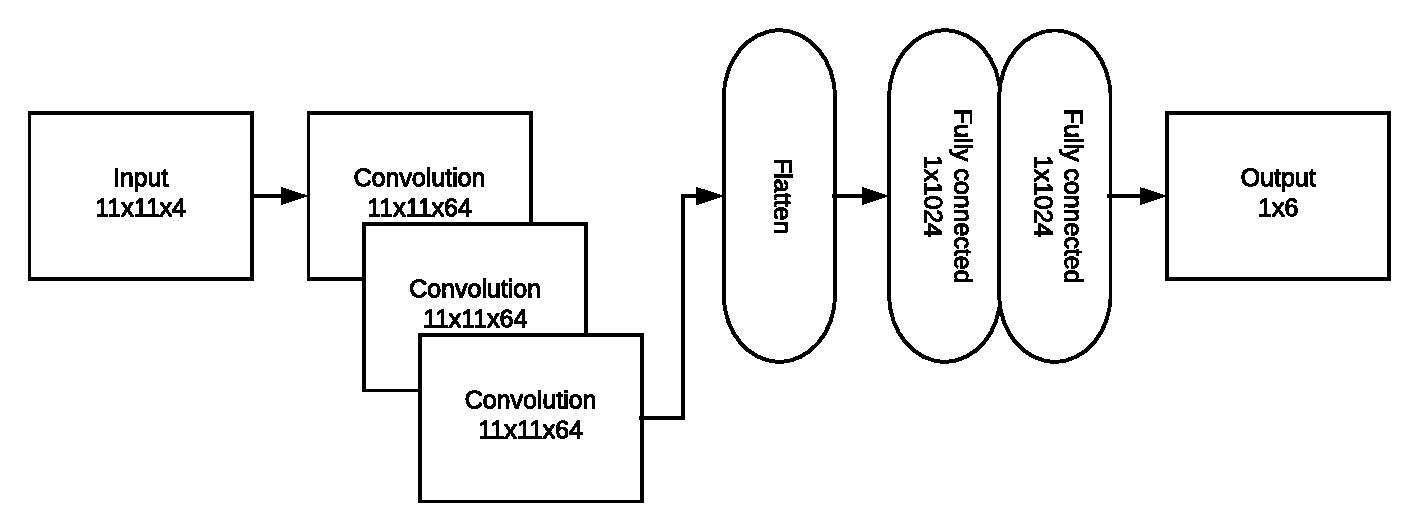
\includegraphics[width=1.0\linewidth]{docs/article/inputs/conv.pdf}}
    \caption{Layout of the neural network}\label{fig:network}
\end{figure}

Some feature engineering has been performed on the input data to reduce complexity (i.e. supplying agent position as sets of coordinates may introduce unnecessary complexity). The state is represented by a $11\times 11\times 4$ tensor in which the following information is conveyed:
\begin{itemize}
    \item A $11\times 11$ tensor conveying obstacle positions
    \item A $11\times 11$ tensor conveying the agent's position
    \item A $11\times 11$ tensor conveying enemy agent positions
    \item A $11\times 11$ tensor conveying \emph{danger zones}
\end{itemize}
The term \emph{danger zones} is referred to as positions in which a bomb will eventually detonate and cause an agent harm. The intention is to represent the state as straightforward as possible to increase learning rates.


\subsection{Exploration / Exploitation}
% The number of possible states in the pommerman environment is enormous
To address the inherent problem in reinforcement learning of exploration versus exploitation while training the agent, was an $\epsilon$-greedy strategy with a decay introduced. The decay is defined as a function $\gamma$ of time.\cite{nieuwdorp2017dare} Adding the $\gamma$ function somewhat allows for control of when the agent should start exploiting what it has learned. In figure~\ref{fig:gamma} are the values of $\epsilon$ illustrated, where it is decayed by two different $\gamma$ functions. In both cases have an initial value of $\epsilon=1$ been used, i.e. the first iteration is $100\%$ random actions.

\begin{figure}[htb]
    \begin{minipage}[b]{.48\linewidth}
        \centering
        \centerline{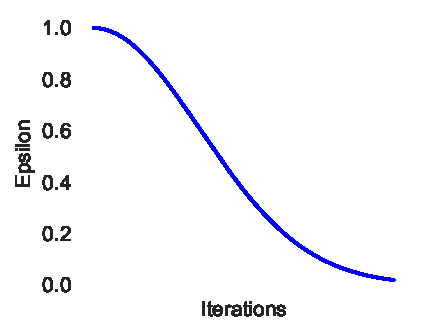
\includegraphics[width=\linewidth]{pommerman/plots/epsilon_8.pdf}}
        \centerline{(a) $\epsilon$ value where $\gamma(x=8)$.}\medskip
    \end{minipage}
    \hfill
    \begin{minipage}[b]{0.48\linewidth}
        \centering
        \centerline{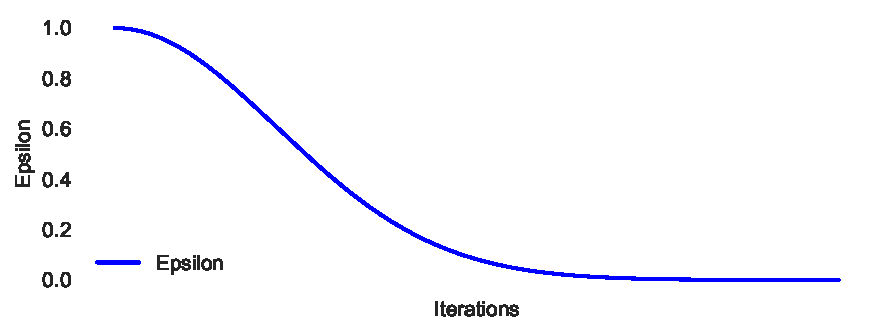
\includegraphics[width=\linewidth]{pommerman/plots/epsilon_20.pdf}}
        \centerline{(b) $\epsilon$ value where $\gamma(x=20)$.}\medskip
    \end{minipage}
    \caption{$\gamma$ = $n / (i / (n / x) + n)$ where $i \in iterations$.}
    \label{fig:gamma}
\end{figure}

(a) is extending the exploration, such that the value of $\epsilon \approx 0$ when approximately $85\%$ of the iterations has been carried out. (b) on the other hand will almost exclusively exploit when approximately $60\%$ of the iterations has been carried out, that is the value of $\epsilon \approx 0$.

% Not completely sure the argument blow is valid as the two graphs have different slopes.
(a) was primarily introduced to maximise the exploration, while keeping the amount of iterations for training at a minimum, as it would require roughly $42\%$ more iterations to achieve the same quantity of exploration with (b).

Another technique that was added in order to try and motivate the agent to explore the map, was to introduce a so called \emph{stop agent}, that would simply perform the action \emph{Stop} all the time. Both the random and simple agents have a probability of blowing themselves up, which will reward our agent with a positive reward if it is the last one standing. If this positive reward is achieved by doing nothing, it could promote the actions that was taken in that iteration thereby increasing the probability for performing a single action. The idea behind having the other agents standing still is that our agent would only be able to achieve a positive reward by exploring the board and potentially blow up its opponents. If all agent are standing still for long enough the game will end in a tie every the agent are rewarded with a negative reward.

\subsection{Static Board}
\label{sec:static}
% Static board to reduce complexity
To reduce the complexity of the search space has the option for keeping the Pommerman board static been introduced for both the training and validation of the network. This is rather than using an new randomly generated board every time a training or validation is carried out as is the case in figure~\ref{fig:pomIntro}. By doing so reduces the number of different boards the agent has to learn to a single board and thereby reducing the total number of possible states tremendously.

\subsection{Reward Function}
% Simple +/-1 1
% Cite bomberman/our tweaked version
Functionality to change the reward function has also been introduced. Besides the standard reward function that comes with the Pommerman environment, where the agents receives a score of 1 for winning and -1 for loosing, some agents were trained with reward shaping. The general motivation for introducing the reward shaping was to encourage the agent to avoid getting stuck in a local minimum. One of the reward functions used for this was the same as was used by \cite{kormelink2018exploration} and can be seen in table~\ref{tab:rew}. 

\begin{table}[htb]
    \centerline{
        \begin{tabular}{|l|r|}
            \hline
            Action                  & Reward   \\ 
            \hline
            Blow up opponent 		& $100$	\\
            Blow up wall  			& $30$  \\
            Perform action			& $-1$	\\
            Perform illegal action	& $-2$	\\
            Die  					& $-300$\\
            \hline
        \end{tabular}
    }
    \caption{A table with an example of reward shaping.}\label{tab:rew}
\end{table}

This specific reward function was introduced in an attempt to encourage the agent to explore the map by rewarding the agent for blowing up wall and giving it negative reward for moving and performing illegal actions, like walking into a wall. In other words if the agent wish to receive a total positive reward it has to blow up opponents or walls.